\clearpage
\section{Materiales y métodos}

\subsection{Estrategia de desarrollo, alternativas y decisiones técnicas}

Siguiendo la metodología de investigación en ciencias del diseño (DSRM) \cite{peffers2007} y el enfoque incremental descritos en el Capítulo 1, el desarrollo se articula en torno a decisiones técnicas que acotan las alternativas existentes en la literatura a los objetivos del trabajo:

\begin{enumerate}
  \item \textbf{Elección del método de referencia frente a estructuras jerárquicas en CPU:} Para obtener un volumen de distancias exacto con el que contrastar la alternativa aproximada, se contemplan dos opciones: construir una jerarquía de volúmenes envolventes (\textit{Bounding Volume Hierarchy}, BVH) en CPU o evaluar directamente los triángulos en GPU mediante \textit{compute shaders} leyendo desde un \textit{buffer} SSBO. Se opta por la evaluación directa masivamente paralela en GPU porque evita la complejidad de mantener y recorrer árboles espaciales con divergencia de ramas en shaders, aprovecha el ancho de banda de memoria de la tarjeta gráfica y garantiza una referencia determinista exacta punto-triángulo en cada centro de vóxel. Antes de emplearlo como referencia sobre escenas complejas, su exactitud se verifica frente a geometrías de control (esfera y cubo) cuyas funciones SDF analíticas son conocidas en forma cerrada.
  \item \textbf{Diseño de la alternativa rápida (captura superficial + JFA 3D):} Para desacoplar la generación del campo del número de triángulos de la malla, se elige combinar una primera fase de extracción de semillas superficiales con una segunda fase de propagación mediante JFA en tres dimensiones ($M = \log_2 V$ pasadas con saltos $k = V / 2^{s+1}$ sobre los 26 vecinos tridimensionales y esquema de doble \textit{buffer} \textit{ping-pong}). Se incluyen también en el estudio las variantes $\text{JFA}+1$ y $1+\text{JFA}$ \cite{rong2006} para cuantificar si el coste de una pasada adicional a distancia unitaria compensa la reducción del error en las fronteras de Voronoi.
  \item \textbf{Estrategia de determinación del signo interior/exterior:} Entre las tres familias revisadas en el estado del arte (pseudo-normales ponderadas por ángulo \cite{baerentzen2005}, conteo de intersecciones por rayos y \textit{Generalized Winding Numbers} \cite{jacobson2013}), se prioriza el trabajo con mallas cerradas o con orientación consistente de caras, combinando la información normal/topológica local con pruebas de paridad o propagación para evitar el coste cuadrático de evaluar ángulos sólidos completos en cada vóxel.
  \item \textbf{Aislamiento y validación progresiva del entorno visual (Hito OE1 y avance OE2):} Un riesgo metodológico habitual al evaluar estructuras geométricas mediante renderizado es confundir los artefactos propios del trazador de rayos o del filtro de ruido con los errores del campo de distancias. Por ello, esta primera fase del visor se estructura en dos pasos incrementales: primero, inyectando primitivas analíticas directamente en la función de distancias del shader para validar el trazador por \textit{sphere tracing} y el filtro SVGF sin errores de discretización; y segundo, añadiendo la visualización de texturas de distancia 3D (\texttt{GL\_TEXTURE\_3D}) generadas también con primitivas analíticas codificadas directamente en un \textit{compute shader} a modo de \textit{placeholder}, listas para ser sustituidas por las texturas generadas a partir de mallas poligonales en las fases posteriores.
\end{enumerate}

\subsection{Herramientas y pila tecnológica}

Para garantizar la portabilidad, el control explícito sobre la memoria de vídeo y la ausencia de dependencias de hardware propietario de trazado de rayos, se selecciona una pila basada en estándares abiertos encabezada por C++20 y OpenGL 4.6 Core Profile. OpenGL 4.6 proporciona soporte nativo para \textit{compute shaders}, acceso aleatorio de lectura y escritura a texturas tridimensionales mediante \texttt{glBindImageTexture} (\texttt{shader\_image\_load\_store}), \textit{buffers} de almacenamiento masivo SSBO con alineamiento \texttt{std430} y consultas asíncronas de tiempo en GPU (\texttt{GL\_TIME\_ELAPSED}). La Tabla~\ref{tab:pila} resume los componentes y herramientas utilizados.

\begin{table}[htbp]
  \centering
  \small
  \caption{Pila tecnológica y entorno de desarrollo.}
  \label{tab:pila}
  \begin{tabularx}{\textwidth}{|>{\bfseries}p{44mm}|>{\raggedright\arraybackslash}p{44mm}|X|}
    \hline
    \rowcolor{tablegray} Componente & Versión / Especificación & Propósito en el proyecto \\ \hline
    Lenguaje de programación & C++20 (ISO/IEC 14882:2020) & Núcleo de la aplicación, gestión de recursos y coordinación del \textit{pipeline} en GPU. \\ \hline
    API Gráfica & OpenGL 4.6 Core Profile / GLSL 4.60 & Ejecución de \textit{compute shaders}, FBOs, texturas 3D, SSBOs y \textit{deferred rendering}. \\ \hline
    SDL3 & Versión 3.2.0 & Creación de ventanas, contexto OpenGL, captura de eventos y temporización. \\ \hline
    GLAD & Especificación Core 4.6 & Carga dinámica de punteros a funciones de OpenGL 4.6 en el host. \\ \hline
    GLM & Versión 1.0.1 & Álgebra lineal tridimensional, matrices de transformación y vectores. \\ \hline
    Assimp & Versión 5.4+ & Importación de mallas tridimensionales (OBJ, glTF), cálculo de normales y AABB. \\ \hline
    Dear ImGui & Versión 1.91.8 & Interfaz gráfica para control de parámetros, diagnóstico e inspección de volúmenes. \\ \hline
    stb\_image / stb\_image\_write & Versión 2.30 / 1.16 & Carga de recursos auxiliares y exportación de capturas sin pérdida. \\ \hline
    RenderDoc & Versión 1.3x & Inspección de texturas 3D, SSBOs, estados del pipeline y depuración de shaders. \\ \hline
    Sistema de compilación & CMake 3.28+ con Ninja & Configuración multiplataforma y compilación incremental. \\ \hline
    Compilador C++ & GCC 14.2 / Clang 18.1 & Generación de código binario nativo optimizado. \\ \hline
    Hardware de pruebas & AMD Radeon RX 9060 XT (RDNA 4) / Mesa 26.2 & Plataforma principal de desarrollo y evaluación en GPU. \\ \hline
  \end{tabularx}
\end{table}

\subsection{Entorno interactivo de validación desarrollado (Hito OE1 y avance OE2)}

Como parte del trabajo realizado hasta esta entrega, se ha implementado y verificado la primera fase del visor interactivo que actuará como banco de pruebas experimental durante todo el proyecto. El desarrollo de este entorno se articula de forma incremental en dos etapas sucesivas: en primer lugar, se implementan primitivas analíticas inyectadas directamente en la función de evaluación de distancias del shader para construir y validar el \textit{path tracer} por \textit{sphere tracing} a 1 muestra por píxel (1 SPP) y la reconstrucción espacio-temporal mediante SVGF \cite{schied2017}; en segundo lugar, se incorpora el soporte y la visualización de texturas tridimensionales de distancia (\texttt{GL\_TEXTURE\_3D}), generadas inicialmente mediante primitivas analíticas codificadas también de forma directa en un \textit{compute shader} a modo de \textit{placeholder}, con el propósito de que sean sustituidas posteriormente por las texturas generadas a partir de mallas poligonales. La Figura~\ref{fig:arquitectura_visor} muestra el flujo de datos entre los distintos pases coordinados por la clase \texttt{renderer::PathTracerPipeline} y la Tabla~\ref{tab:fbos} detalla los \textit{Framebuffer Objects} (FBO) y texturas asociados.

\begin{figure}[htbp]
  \centering
  \begin{tikzpicture}[
    node distance=7mm and 10mm,
    font=\small\sffamily,
    basebox/.style={draw=black, line width=0.6pt, align=center, inner sep=5pt},
    inputbox/.style={basebox, fill=uoccyan!20, text width=52mm},
    passbox/.style={basebox, fill=white, rounded corners=3pt, text width=70mm, line width=0.8pt},
    mrtbox/.style={basebox, fill=tablegray, text width=70mm},
    outbox/.style={basebox, fill=uocblue!10, text width=60mm, line width=0.8pt},
    histbox/.style={basebox, fill=uoccyan!10, dashed, text width=32mm},
    arr/.style={->, >=Latex, line width=0.8pt}
  ]
    % Inputs
    \node[inputbox] (inputA) {Primitivas Analíticas\\en Shader};
    \node[inputbox, right=14mm of inputA] (inputB) {Textura 3D SDF\\(\textit{Placeholder} GPU)};

    % Center coordinate
    \coordinate (inMid) at ($(inputA.south)!0.5!(inputB.south)$);

    % Pass 1
    \node[passbox, below=9mm of inMid] (pass1) {\textbf{Pase 1: Path Tracer SDF}\\(1-SPP Sphere Tracing)};

    % MRT
    \node[mrtbox, below=7mm of pass1] (mrt) {\textbf{MRT Primario (4 Targets)}\\Illum (Demod), Norm, Pos, Albedo};

    % Pass 2A
    \node[passbox, below=7mm of mrt] (pass2a) {\textbf{Pase 2A: SVGF Temporal}\\Reproyección + Momentos};
    \node[histbox, right=10mm of pass2a] (hist) {Historial $t-1$};

    % Pass 2B
    \node[passbox, below=7mm of pass2a] (pass2b) {\textbf{Pase 2B: SVGF À-Trous}\\4 Pasadas Ping-Pong ($2^i$)};

    % Pass 3
    \node[passbox, below=7mm of pass2b] (pass3) {\textbf{Pase 3: Resolve}\\Re-modulación Albedo + Gamma sRGB / Debug};

    % Output
    \node[outbox, below=7mm of pass3] (output) {\textbf{Pantalla / FBO Salida}};

    % Arrows
    \draw[arr] (inputA.south) |- ++(0,-3mm) -| (pass1.north);
    \draw[arr] (inputB.south) |- ++(0,-3mm) -| (pass1.north);
    \draw[arr] (pass1) -- (mrt);
    \draw[arr] (mrt) -- (pass2a);
    \draw[arr] (hist) -- (pass2a);
    \draw[arr] (pass2a) -- (pass2b);
    \draw[arr] (pass2b) -- (pass3);
    \draw[arr] (pass3) -- (output);
  \end{tikzpicture}
  \caption{Arquitectura del banco de pruebas visual con evaluación de SDF y reducción de ruido SVGF.}
  \label{fig:arquitectura_visor}
\end{figure}

\begin{table}[htbp]
  \centering
  \small
  \caption{Configuración de recursos volumétricos y Framebuffer Objects (FBO) en el visor de validación.}
  \label{tab:fbos}
  \begin{tabularx}{\textwidth}{|>{\bfseries\raggedright\arraybackslash}p{34mm}|>{\raggedright\arraybackslash}p{21mm}|>{\raggedright\arraybackslash}p{21mm}|>{\raggedright\arraybackslash}p{24mm}|X|}
    \hline
    \rowcolor{tablegray} Recurso / FBO & Attachment & Textura & Formato interno & Datos almacenados \\ \hline
    \texttt{m\_sdfTexture} & Imagen / Sampler & \texttt{Texture3D} & \texttt{GL\_R32F} & Campo de distancias 3D generado en \textit{compute shader} (\textit{placeholder}). \\ \hline
    \texttt{m\_primaryFbo} & Color 0--3 & \texttt{m\_primary*} & \texttt{GL\_RGBA16F} & Irradiancia demodulada, profundidad lineal, normal, impacto y albedo. \\ \hline
    \texttt{m\_temporalFbo[2]} & Color 0--1 & \texttt{m\_temporal*} & \texttt{GL\_RGBA16F} & Irradiancia integrada, varianza temporal, momentos ($\mu_1, \mu_2$) y longitud de historial. \\ \hline
    \texttt{m\_atrousPing/} \newline \texttt{Pong} & Color 0 & \texttt{m\_atrous*} & \texttt{GL\_RGBA16F} & Irradiancia y varianza filtradas mediante filtro \textit{wavelet} À-Trous ($5\times 5$). \\ \hline
  \end{tabularx}
\end{table}

El funcionamiento de esta primera fase del entorno de pruebas comprende los siguientes mecanismos clave:

\begin{itemize}
  \item \textbf{Evaluación con primitivas analíticas y muestreo con ruido azul (STBN):} En el primer paso de implementación del visor (\texttt{sdf\_raymarching.\allowbreak frag}), las escenas de prueba (como la caja de Cornell y el muestrario de materiales) se definen inyectando primitivas SDF analíticas (esferas, cajas, cilindros y planos combinados mediante operaciones booleanas) directamente en la función de distancias del shader (\texttt{fScene}). A partir de la intersección primaria obtenida por \textit{sphere tracing}, se evalúa la iluminación directa con sombras suaves cónicas y un rebote indirecto (difuso por muestreo coseno o especular gobernado por Fresnel-Schlick \cite{karis2013}). Para evitar la aglomeración de ruido en bajas frecuencias propia de los generadores pseudoaleatorios de ruido blanco (PCG), se integran máscaras de ruido azul espaciotemporal (\textit{Spatiotemporal Blue Noise}, STBN) \cite{wolfe2022egsr, wolfe2022nv} almacenadas en texturas 3D de $128 \times 128 \times 64$ texeles, que distribuyen el error estocástico en frecuencias altas fácilmente suprimibles por el filtro posterior.
  \item \textbf{Visualización de texturas de distancia 3D a modo de \textit{placeholder} (avance del Hito OE2):} Una vez validado el trazador con ecuaciones directas en el shader, se incorpora el soporte para almacenar y muestrear campos de distancia discretos en texturas tridimensionales mediante las clases \texttt{Texture3D} y \texttt{ComputeShader} junto con el shader \texttt{generate\_3d\_sdf.\allowbreak comp}. En esta fase, dicho \textit{compute shader} rellena texturas \texttt{GL\_TEXTURE\_3D} en formato \texttt{GL\_R32F} (a resoluciones configurables de $32^3$ a $256^3$) evaluando también primitivas analíticas codificadas directamente en el propio shader (una esfera de 1 m de diámetro, un conjunto de primitivas y una habitación hueca con ventana mediante operaciones CSG). Estas texturas actúan como \textit{placeholder} funcional para dejar resueltos y verificados el muestreo trilineal continuo en hardware, el cálculo de normales por diferencias centrales adaptadas al tamaño de vóxel (\texttt{get3DTextureNormal}) y el \textit{surface bias} proporcional a la resolución (\texttt{getSurfaceBias}), de modo que en la siguiente fase puedan sustituirse de forma transparente por las texturas generadas a partir de mallas poligonales.
  \item \textbf{Reconstrucción espacio-temporal SVGF estabilizada:}\par El pase temporal (\texttt{svgf\_temporal.\allowbreak frag}) reproyecta las muestras mediante la matriz del fotograma anterior validando la coherencia de normales, distancia planar y continuidad de superficie, y actualiza la media exponencial junto con los momentos de luminancia ($\mu_1, \mu_2$). En regiones recién desocluidas con historial corto, complementa la estimación de varianza con un vecindario espacial bilateral de $7 \times 7$. A continuación, el filtro espacial (\texttt{svgf\_atrous.\allowbreak frag}) aplica cuatro iteraciones \textit{ping-pong} con núcleo $B_3$-spline de $5 \times 5$ y pasos $s \in \{1, 2, 4, 8\}$ \cite{dammertz2010}, ponderadas por funciones de preservación de bordes (\textit{edge-stopping functions}) de normal, profundidad planar y luminancia, antes de remodular el albedo y aplicar la corrección gamma en \texttt{linear\_to\_srgb.\allowbreak frag}.
  \item \textbf{Interfaz diagnóstica y verificación del visor:} La interfaz en Dear ImGui permite alternar escenas, configurar luces, cámara y escala de resolución, conmutar entre la evaluación analítica directa y la lectura de la textura 3D \textit{placeholder} a distintas resoluciones, e inspeccionar seis vistas diagnósticas (imagen final reconstruida, entrada bruta a 1 SPP, irradiancia filtrada (\textit{denoised}), varianza estimada, normales y albedo). Sobre una GPU AMD Radeon RX 9060 XT a resolución de $960 \times 540$, el filtro SVGF completo consume aproximadamente \textbf{1,85 ms} por fotograma, manteniendo tasas superiores a \textbf{120 FPS}, y supera la batería automatizada \texttt{--test} con \textbf{0 píxeles anómalos (\texttt{NaN}/\texttt{Inf})}. Tal como muestran la Figura~\ref{fig:cornell_box} y la Figura~\ref{fig:primitivas_sdf}, el visor reproduce con fidelidad tanto la transferencia indirecta de color (\textit{color bleeding}) en la caja de Cornell como las sombras suaves y reflexiones sobre geometría SDF.
\end{itemize}

\begin{figure}[htbp]
  \centering
  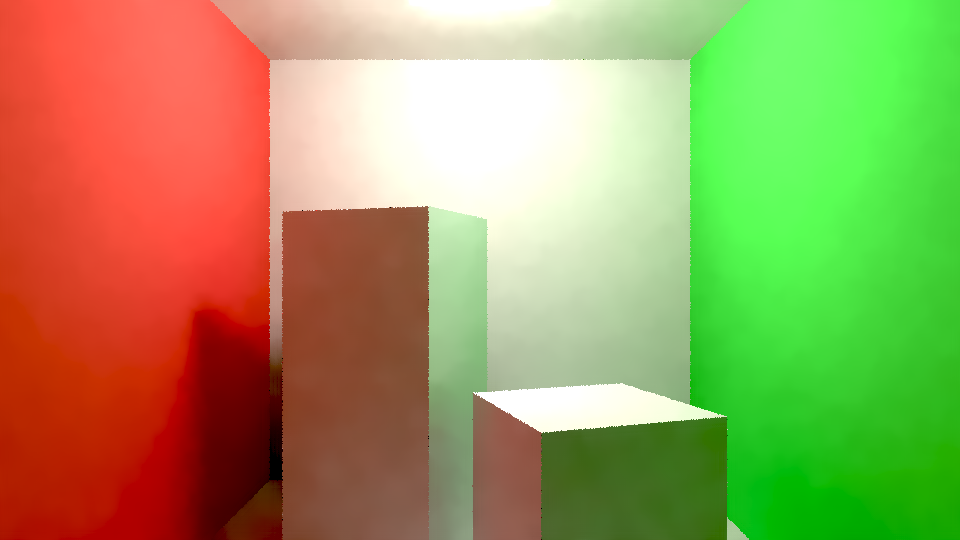
\includegraphics[width=0.78\textwidth]{docs/assets/scene1_denoised.png}
  \caption{Escena de validación Cornell Box renderizada en tiempo real en el visor a 1 muestra por píxel con reconstrucción SVGF.}
  \label{fig:cornell_box}
\end{figure}

\begin{figure}[htbp]
  \centering
  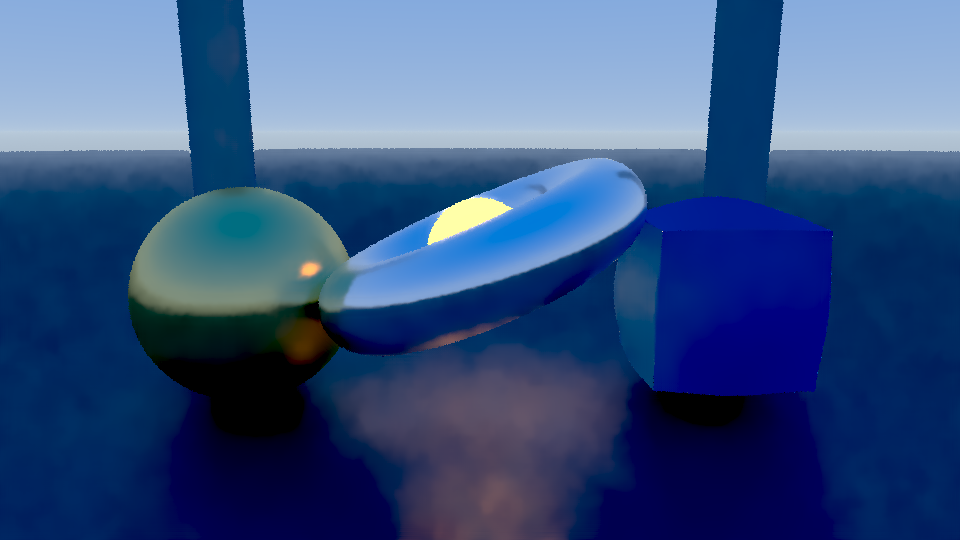
\includegraphics[width=0.78\textwidth]{docs/assets/scene2_slate_floor.png}
  \caption{Escena de validación con muestrario de primitivas SDF, reflexiones especulares y sombras suaves.}
  \label{fig:primitivas_sdf}
\end{figure}

\subsection{Escenas de evaluación y protocolo experimental}

Para la evaluación comparativa de los dos métodos de generación de SDF a partir de mallas poligonales (que se ejecutará en las fases correspondientes a las entregas PEC 3 y PEC 4), se definen los siguientes modelos de entrada y métricas de análisis:

\subsubsection{Modelos y escenas poligonales de prueba}

\begin{enumerate}
  \item \textbf{Modelos geométricos de control (Esfera y Cubo poligonales):} Mallas sintéticas cerradas teseladas con densidad poligonal variable ($1.000$ a $20.000$ triángulos) cuyas dimensiones coinciden con funciones SDF analíticas conocidas en forma cerrada:
  \begin{equation}
    f_{\text{esfera}}(p) = \|p\| - r, \quad f_{\text{cubo}}(p) = \|\max(|p| - b, 0)\| + \min(\max(|p| - b), 0)
  \end{equation}
  Estas geometrías permitirán comprobar numéricamente la exactitud del generador base en \textit{compute shaders} antes de emplear sus volúmenes como referencia.
  \item \textbf{Cornell Box poligonal:} Versión discretizada en triángulos de la caja de Cornell tradicional, utilizada para evaluar el comportamiento de ambos generadores en recintos cerrados con ángulos diedros rectos y oclusiones controladas.
  \item \textbf{Crytek Sponza:} Escena arquitectónica compuesta por aproximadamente $262.000$ triángulos con arcos, columnas y detalles geométricos complejos, destinada a evaluar la escalabilidad temporal y el consumo de memoria ante un número elevado de primitivas.
\end{enumerate}

\subsubsection{Protocolo de medición y métricas cuantitativas}

Los dos generadores se compararán bajo condiciones idénticas de GPU, formato de almacenamiento (\texttt{GL\_R16F} y \texttt{GL\_R32F}) y resolución volumétrica ($64^3, 128^3$ y $256^3$ vóxeles), registrando tres métricas principales:

\begin{enumerate}
  \item \textbf{Tiempo de generación en GPU (ms):} Se aislará el tiempo de ejecución de los \textit{compute shaders} de generación respecto a la CPU y al renderizado del visor mediante objetos de consulta asíncrona de OpenGL (\texttt{GL\_TIME\_ELAPSED}).
  \item \textbf{Consumo de memoria de vídeo VRAM (MB):} Se contabilizará la memoria estática ocupada por la textura volumétrica de salida (\texttt{GL\_TEXTURE\_3D}) junto con la memoria temporal adicional requerida durante la generación (\textit{buffers} SSBO de geometría y texturas \textit{ping-pong} de coordenadas de semillas en JFA 3D).
  \item \textbf{Error numérico del campo de distancias:} Tomando el volumen generado por el método base de cálculo exacto punto-triángulo como campo de referencia $f_{\text{ref}}(i, j, k)$, se evaluarán vóxel a vóxel sobre los $V^3$ elementos de la cuadrícula las siguientes métricas de discrepancia frente al volumen obtenido mediante JFA $f_{\text{JFA}}(i, j, k)$:
  \begin{itemize}
    \item \textbf{Error Absoluto Medio (MAE, \textit{Mean Absolute Error}):}
    \begin{equation}
      \text{MAE} = \frac{1}{V^3} \sum_{i=1}^{V_x} \sum_{j=1}^{V_y} \sum_{k=1}^{V_z} \left| f_{\text{JFA}}(i, j, k) - f_{\text{ref}}(i, j, k) \right|
    \end{equation}
    \item \textbf{Error Cuadrático Medio (RMSE, \textit{Root Mean Square Error}):}
    \begin{equation}
      \text{RMSE} = \sqrt{\frac{1}{V^3} \sum_{i=1}^{V_x} \sum_{j=1}^{V_y} \sum_{k=1}^{V_z} \left( f_{\text{JFA}}(i, j, k) - f_{\text{ref}}(i, j, k) \right)^2}
    \end{equation}
    \item \textbf{Error Máximo Absoluto ($E_{\max}$):}
    \begin{equation}
      E_{\max} = \max_{i, j, k} \left| f_{\text{JFA}}(i, j, k) - f_{\text{ref}}(i, j, k) \right|
    \end{equation}
  \end{itemize}
\end{enumerate}
